

\tikzset{every picture/.style={line width=0.75pt}} %set default line width to 0.75pt        

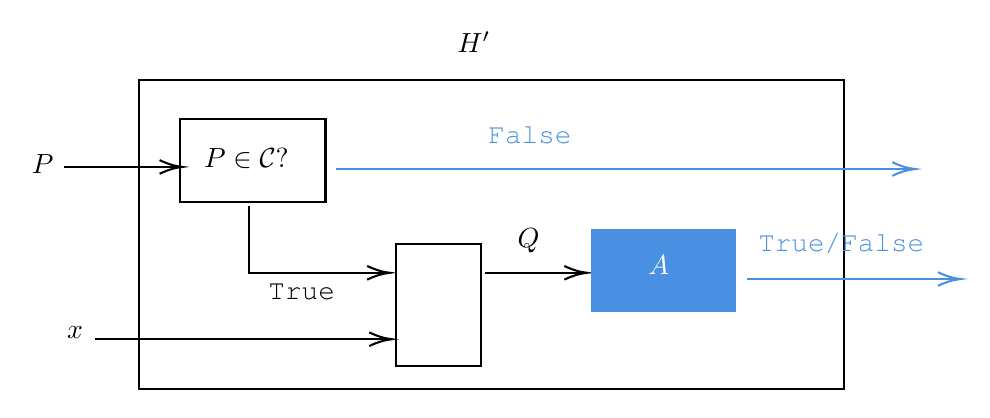
\begin{tikzpicture}[x=0.75pt,y=0.75pt,yscale=-1,xscale=1]
%uncomment if require: \path (0,300); %set diagram left start at 0, and has height of 300

%Shape: Rectangle [id:dp13757980277427873] 
\draw   (160,62) -- (500,62) -- (500,211) -- (160,211) -- cycle ;
%Shape: Rectangle [id:dp4459702690538667] 
\draw   (180,81) -- (250,81) -- (250,121) -- (180,121) -- cycle ;
%Straight Lines [id:da7388620921419784] 
\draw    (124,104) -- (179,104) ;
\draw [shift={(181,104)}, rotate = 180] [color={rgb, 255:red, 0; green, 0; blue, 0 }  ][line width=0.75]    (10.93,-3.29) .. controls (6.95,-1.4) and (3.31,-0.3) .. (0,0) .. controls (3.31,0.3) and (6.95,1.4) .. (10.93,3.29)   ;
%Straight Lines [id:da653111356612567] 
\draw    (213,123) -- (213,155) -- (279,155) ;
\draw [shift={(281,155)}, rotate = 180] [color={rgb, 255:red, 0; green, 0; blue, 0 }  ][line width=0.75]    (10.93,-3.29) .. controls (6.95,-1.4) and (3.31,-0.3) .. (0,0) .. controls (3.31,0.3) and (6.95,1.4) .. (10.93,3.29)   ;
%Shape: Rectangle [id:dp06756433291766983] 
\draw   (284,141) -- (325,141) -- (325,200) -- (284,200) -- cycle ;
%Straight Lines [id:da7593586995464512] 
\draw    (327,155) -- (374,155) ;
\draw [shift={(376,155)}, rotate = 180] [color={rgb, 255:red, 0; green, 0; blue, 0 }  ][line width=0.75]    (10.93,-3.29) .. controls (6.95,-1.4) and (3.31,-0.3) .. (0,0) .. controls (3.31,0.3) and (6.95,1.4) .. (10.93,3.29)   ;
%Shape: Rectangle [id:dp3284906616989065] 
\draw  [draw opacity=0][fill={rgb, 255:red, 74; green, 144; blue, 226 }  ,fill opacity=1 ] (378,134) -- (448,134) -- (448,174) -- (378,174) -- cycle ;
%Straight Lines [id:da949118748450994] 
\draw    (139,187) -- (280,187) ;
\draw [shift={(282,187)}, rotate = 180] [color={rgb, 255:red, 0; green, 0; blue, 0 }  ][line width=0.75]    (10.93,-3.29) .. controls (6.95,-1.4) and (3.31,-0.3) .. (0,0) .. controls (3.31,0.3) and (6.95,1.4) .. (10.93,3.29)   ;
%Straight Lines [id:da8301177238692266] 
\draw [color={rgb, 255:red, 74; green, 144; blue, 226 }  ,draw opacity=1 ]   (255,105) -- (532,105) ;
\draw [shift={(534,105)}, rotate = 180] [color={rgb, 255:red, 74; green, 144; blue, 226 }  ,draw opacity=1 ][line width=0.75]    (10.93,-3.29) .. controls (6.95,-1.4) and (3.31,-0.3) .. (0,0) .. controls (3.31,0.3) and (6.95,1.4) .. (10.93,3.29)   ;
%Straight Lines [id:da07628925478688586] 
\draw [color={rgb, 255:red, 74; green, 144; blue, 226 }  ,draw opacity=1 ]   (453,158) -- (554,158) ;
\draw [shift={(556,158)}, rotate = 180] [color={rgb, 255:red, 74; green, 144; blue, 226 }  ,draw opacity=1 ][line width=0.75]    (10.93,-3.29) .. controls (6.95,-1.4) and (3.31,-0.3) .. (0,0) .. controls (3.31,0.3) and (6.95,1.4) .. (10.93,3.29)   ;

% Text Node
\draw (190,93.4) node [anchor=north west][inner sep=0.75pt]    {$P\in \mathcal{C} ?$};
% Text Node
\draw (107,96.4) node [anchor=north west][inner sep=0.75pt]    {$P$};
% Text Node
\draw (221,159) node [anchor=north west][inner sep=0.75pt]   [align=left] {{\fontfamily{pcr}\selectfont True}};
% Text Node
\draw (124,179.4) node [anchor=north west][inner sep=0.75pt]    {$x$};
% Text Node
\draw (404,145.4) node [anchor=north west][inner sep=0.75pt]  [color={rgb, 255:red, 255; green, 255; blue, 255 }  ,opacity=1 ]  {$A$};
% Text Node
\draw (341,132.4) node [anchor=north west][inner sep=0.75pt]    {$Q$};
% Text Node
\draw (327,83) node [anchor=north west][inner sep=0.75pt]  [color={rgb, 255:red, 74; green, 144; blue, 226 }  ,opacity=1 ] [align=left] {{\fontfamily{pcr}\selectfont False}};
% Text Node
\draw (457,135) node [anchor=north west][inner sep=0.75pt]  [color={rgb, 255:red, 74; green, 144; blue, 226 }  ,opacity=1 ] [align=left] {{\fontfamily{pcr}\selectfont True/False}};
% Text Node
\draw (312,37.4) node [anchor=north west][inner sep=0.75pt]    {$H'$};


\end{tikzpicture}